\documentclass[UTF8]{ctexart}
\usepackage{amsmath}
\usepackage{amssymb}
\usepackage{booktabs}
\usepackage{background}
\usepackage{caption, subcaption}
\usepackage{circuitikz}
\usepackage{enumitem}
\usepackage{float}
\usepackage{fourier}
\usepackage{fontspec}
\usepackage{geometry}
\usepackage{pifont}
\usepackage{tikz}
\usepackage{ulem}
\usepackage{xcolor}
\usetikzlibrary{arrows.meta}



%\backgroundsetup{contents=
\includegraphics{示例.png}, center, scale=1, angle=0, opacity=1}
\geometry{a5paper, top=0.1cm, left=1cm, right=1cm, bottom=1.1cm}
\setCJKmainfont[BoldFont={汉仪文黑-85W},ItalicFont={方正苏新诗柳楷简体}]{汉仪文黑-55W}
\setfontfamily\Issue{Century Schoolbook}
\newCJKfontfamily\TitleFont{思源宋体 CN Heavy}
\newfontfamily\timesnewroman{Times New Roman}
\captionsetup{font=small, labelfont=bf}

\colorlet{darkcyan}{cyan!50!black}
\newcommand\Black[1]{\textcolor[gray]{0.3}{#1}}
\newcommand\Brown[1]{\textcolor[HTML]{998A4E}{#1}}
\newcommand\Emph[1]{\colorbox{cyan!10!}{\textcolor{cyan!50!black}{#1}}}
\newcommand\Correct[1]{\colorbox{green!20}{\textcolor{green!50!black}{#1}}}
\newcommand\mypi{\text{\timesnewroman π}}
%这4个信息随“刊号”更新
\newcommand\IssueNumber{12}
\newcommand\Date{2023-12-4}
%\newcommand\Contributer{@金光日}
\newcommand\Subject{模拟电子线路}
\renewcommand\thefootnote{\ding{\numexpr171 + \value{footnote}}}
\newcommand\xb[1]{_\mathrm{#1}}

\newcommand\amp[1]{\colorbox{cyan!10}{\textcolor{cyan}{#1}}}
\newcommand\fre[1]{\colorbox{green!10}{\textcolor{green!60!black}{#1}}}

\ctikzset{
    bipoles/length=0.8cm,
    resistors/scale=0.6, % smaller R
    capacitors/scale=0.6, % even smaller C
    diodes/scale=0.5, % small diodes
    transistors/scale=0.65,
    sources/scale=0.7,
    csources/scale=0.6,
    batteries/scale=0.5,
    grounds/scale=0.5,
    amplifiers/scale=0.7, amplifiers/plus={\scriptsize $+$}, amplifiers/minus={\scriptsize $-$},
    current arrow scale=24, % 数值越大箭头越小
}

\begin{document}
\backgroundsetup{contents=
\includegraphics{上半示例.png}, center, scale=1, angle=0, opacity=1}
\BgThispage
\begin{center}
{\scriptsize\Issue \textcolor[HTML]{C8BA83}{WEEKLY TIPS}}

{\Huge\bfseries\TitleFont \Black{知\ 识\ 小\ 料}}

\vspace{-0.1cm}
{\footnotesize \Brown{「电计 2203 班」周常规知识整理共享}}
\end{center}

\vspace{-0.5cm}

\begin{figure}[H]
\hspace{1cm}
\begin{minipage}[t]{0.3\textwidth}
\centering
    \Brown{ISSUE.}

    \vspace{-0.6cm}
    \Huge \Issue\slshape\bfseries\Black{\IssueNumber}
\end{minipage}
\hfill
\begin{minipage}[t]{0.3\textwidth}
\centering
    \Brown{日期:\Date} \\
%\vspace{-0.1cm}
%    \Brown{贡献者:\Contributer} \\
\vspace{-0.1cm}
    \Brown{学科:\Subject} \\
\end{minipage}
\hspace{0.8cm}
\end{figure}

%此处以后填写正文
{\color{cyan!50!black}
图中 $R_2$ 电阻调节范围为 $0\sim 100\mathrm{k\Omega}$,分析电路回答以下问题。
\begin{figure}[htb]
\color{cyan!50!black}
\begin{minipage}[c]{0.4\textwidth}
    \vspace{0cm}
    \begin{enumerate}[itemsep=0pt,parsep=0pt]
      \item 请简要分析电路中正、负反馈的作用?(2分)
      \item 求输出电压的振荡频率的调节范围。(3分)
      \item 求 $R\xb{ab}$ 的下限值。(3分)
      \item 请给出一种稳幅方案。(2分)
    \end{enumerate}
\end{minipage}
\begin{minipage}[c]{0.6\textwidth}
    \centering
    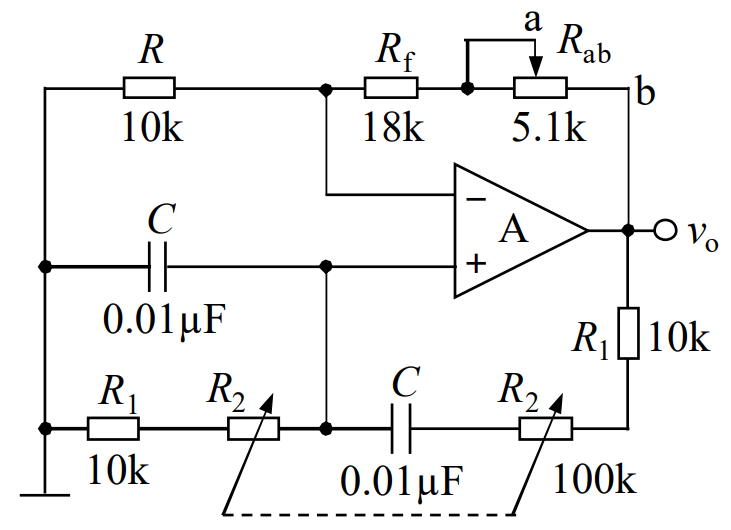
\includegraphics[width=6cm]{题目.png}
\end{minipage}
\end{figure}
}

分析题目和电路图可知,本题有电容、电阻串并联的现象,而且题中出现了“正、负反馈”、“稳幅”等字样,这都是 $RC$ 正弦信号振荡电路的特征,因此初步判定此题考察\textbf{ $RC$ 正弦信号振荡电路}。

\begin{figure}[htb]
    \centering
    \begin{circuitikz}[european,scale=1.5]
        \fill[green!10] (-2.5, -1.4) rectangle (-1.2, 1.1);
        \fill[cyan!10] (-1.2, -1.4) rectangle (1.1, 1.1);
        %\draw[dashed,cyan] (-1.2, -1.3) to (-1.2, 1.1) node[left] {$F$} node[right] {$A$};
        \node[below left, green!60!black] at (-1.2, 1.1) {$F$};
        \node[below right, cyan] at (-1.2, 1.1) {$A$};
        \draw (0,0) node[op amp] (A) {};
        \draw (-2, 1) to[R, l=$R$] (-2, 0.3) to[capacitor, l=$C$] (-2, -0.1) to[short, -*] (-2, -0.3) to (-2.3, -0.3) to[R, l=$R$] (-2.3, -1.1) to[short, -*] (-2, -1.1) to (-2,-1.2) node[rground] {};
        \draw (-2, -0.3) to (-1.7, -0.3) to[capacitor, l=$C$] (-1.7,-1.1) to (-2, -1.1);

        \draw (A.-) to[short, -*] ++(-0.3, 0) coordinate(B) to[short, -*, R, l_=$R_3$] ++(0, 0.86);
        \draw (B) to ++(0, -0.2) to[R, l=$R_4$] ++(0, -1.2) node[rground] {};
        \draw (-2, 1) to (0.6, 1) to[short, -*] (0.6, 0);
        \draw (A.out) to[short, -o] (0.9,0) node[above] {$v\xb{o}$};
        \draw (A.+) to[short, -*] (-2, -0.12);
        \filldraw[fill=white, draw=darkcyan] (-1.2, -0.12) circle (1pt) node[above, color=darkcyan] {$v\xb{i}$};
    \end{circuitikz}
\end{figure}

这是我们上课学过的 $RC$ 正弦信号振荡器的结构,分为\amp{负反馈放大 $(A)$}、\fre{正反馈选频 $(F)$}、稳幅电路\textbf{三部分}。由此便可以回答【第 1 题】:正反馈的作用是选频;负反馈的作用是电压放大,并使电路起振。

【第 2 题】观察题干电路的\fre{选频 $(F)$ 部分},可以发现 $R_1,R_2,C$ 出现两次,且 $R_1,R_2$ 串联构成一个整体,与 $C$ 分别进行串、并联。输入电压 $v\xb{i}$ 在运放的同相端 $(+)$。由选频公式,可知
\begin{equation}\label{eq:frequency}
    f\xb{o} = \dfrac{1}{2\mypi C(R_1+R_2)}
\end{equation}

\newpage
\backgroundsetup{contents=
\includegraphics{下半示例.png}, center, scale=1, angle=0, opacity=1}
\BgThispage

$C$ 和 $R_1$ 都是定值,$R_2$ 取 $0\sim 100\mathrm{k\Omega}$,因此 $f\xb{o}$ 也是变化的数值。取 $R_2=0$,则 $f\xb{o} \approx 1\,591.55\mathrm{Hz}$;取 $R_2=100\mathrm{k\Omega}$,则 $f\xb{o} \approx 144.69\mathrm{k\Omega}$。因此范围就得到了。

【第 3 题】观察题干电路的\amp{放大 $(A)$ 部分},可以发现 $R,R\xb{f},R\xb{ab}$ 构成负反馈放大电路。放大器是一个同相放大器(因为 $v\xb{i}$ 在同相端)。从反相端 $(-)$ 出来两条支路:一条过 $R\xb{f},R\xb{ab}$ 到达输出端 $v\xb{o}$,另一条过 $R$ 到地。因此使用同相放大器的 $A_{v\mathrm{f}}$ 公式可得
\begin{equation}\label{eq:amplifier}
    A_{v\mathrm{f}} = 1 + \dfrac{R\xb{f}+R\xb{ab}}{R} \geqslant 3
\end{equation}
由 $F=\dfrac13$,要让电路起振需 $|AF|\geqslant 1$ 即 $A_{v\mathrm{f}}\geqslant 3$,解不等式得 $R\xb{ab}\geqslant 2\mathrm{k\Omega}$,因此下限值得到。

【第 4 题】观察 $A_{v\mathrm{f}}$ 公式 \eqref{eq:amplifier},要稳定 $A_{v\mathrm{f}}$ ,需要稳定 $R\xb{f},R$(变化的 $R\xb{ab}$ 不用考虑),因此可以把 $R\xb{f},R$ 换成温敏电阻。

\begin{figure}[htb]
    \centering
    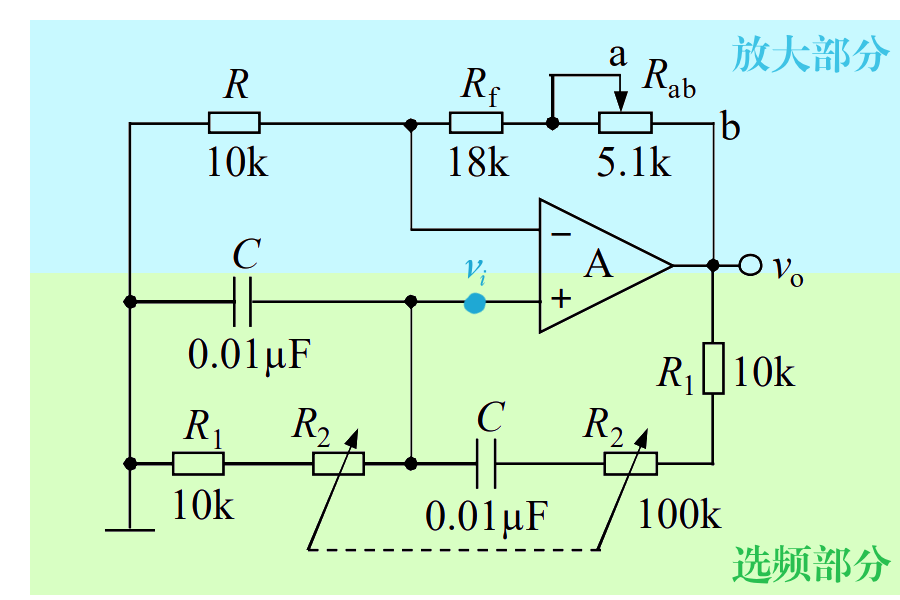
\includegraphics[width=7cm]{题解.png}
\end{figure}
对原题电路拆解以后得到的电路如上图。

{\color{cyan!80!black} 【结论】
\begin{enumerate}[itemsep=0pt, parsep=0pt]
\color{cyan!80!black}
    \item 正反馈选频,负反馈放大,并使电路起振。
    \item 调节范围为 $144.69\mathrm{Hz} \sim 1\,591.55\mathrm{Hz}$。
    \item $R\xb{ab}$ 下限值为 $2\mathrm{k\Omega}$。
    \item 采用温敏电阻。
\end{enumerate}

【点评】本题考察 $RC$ 正弦信号振荡电路的知识,属于后期学习的内容,或许难以定位知识点。而且,本题题干电路变形较大,且构成选频网络的电阻是 $R_1+R_2$ 串联,可能不一定能识别出来。通过学过的电路迁移至考试电路进行解题,是一个好办法。
}

\end{document}